\let\negmedspace\undefined
\let\negthickspace\undefined
\documentclass[journal,12pt,twocolumn]{IEEEtran}
\usepackage{cite}
\usepackage{amsmath,amssymb,amsfonts,amsthm}
\usepackage{algorithmic}
\usepackage{graphicx}
\usepackage{textcomp}
\usepackage{xcolor}
\usepackage{txfonts}
\usepackage{listings}
\usepackage{enumitem}
\usepackage{mathtools}
\usepackage{gensymb}
\usepackage{comment}
\usepackage[breaklinks=true]{hyperref}
\usepackage{tkz-euclide} 
\usepackage{listings}
\usepackage{gvv}                                        
\def\inputGnumericTable{}                                 
\usepackage[latin1]{inputenc}                                
\usepackage{color}                                            
\usepackage{array}                                            
\usepackage{longtable}                                       
\usepackage{calc}                                             
\usepackage{multirow}                                         
\usepackage{hhline}                                           
\usepackage{ifthen}                                           
\usepackage{lscape}
\newtheorem{theorem}{Theorem}[section]
\newtheorem{problem}{Problem}
\newtheorem{proposition}{Proposition}[section]
\newtheorem{lemma}{Lemma}[section]
\newtheorem{corollary}[theorem]{Corollary}
\newtheorem{example}{Example}[section]
\newtheorem{definition}[problem]{Definition}
\newcommand{\BEQA}{\begin{eqnarray}}
\newcommand{\EEQA}{\end{eqnarray}}
\newcommand{\define}{\stackrel{\triangle}{=}}
\theoremstyle{remark}
\newtheorem{rem}{Remark}
\begin{document}
\bibliographystyle{IEEEtran}
\vspace{3cm}
\title{NCERT 11.9.2 16Q}
\author{EE23BTECH11021 - GANNE GOPI CHANDU$^{*}$% <-this % stops a space
}
\maketitle
\newpage
\bigskip
\renewcommand{\thefigure}{\theenumi}
\renewcommand{\thetable}{\theenumi}
\bibliographystyle{IEEEtran}
\textbf{Question}\\
Between 1 and 31, m numbers have been inserted in such a way that the resulting sequence is an A.P. and 
the ratio of 7
th and (m - 1)
th numbers is 5:9. Find the value of m.\\
\textbf{Solution}\\
\begin{table}[h!]
\begin{center}
\renewcommand\thetable{1}
\begin{tabular}{ |c|c|  } 
  \hline
    Parameter & Value  \\ 
  \hline
  First term of A.P $x(0)$ & 1  \\ 
  \hline
  Common difference (d) & 2 \\ 
  \hline
  The value of m & 14 \\
  \hline
  General term x(n) & (2n-1)u(n)\\
  \hline
\end{tabular}
\end{center}
\caption{}
\end{table}
\begin{align}
\text{First term } x(0) &= 1\\
\text{last term } x(n) &= 31\\
\text{number of terms}( n) &= m + 2.
\end{align}
From 1,2,3
\begin{align}
x(n)&=x(0)+nd\\
31 &= 1 + \brak{m + 1}d \\
30 &= \brak{m + 1}d \\
\frac{30}{m + 1} &= d 
\end{align}
Now $7$th and $\brak{m-1}$th terms
\begin{align}
\implies x_7 &= x(0) + 7d   \\ 
\implies x_{m-1} &= x(0) + \brak{m-1}d  
\end{align}
Given that
\begin{align}
\frac{x_{7}}{x_{m-1}} = \frac{5}{9} 
\end{align}
From 5 and 6:
\begin{align}
\implies \frac{x(0) + 7d}{x(0) + \brak{m-1}d} &= \frac{5}{9} 
\end{align}
From 4 and 9:
\begin{align}
\implies \frac{1+7\brak{{\frac{30}{m+1}}}}{1+\brak{{m-1}}\brak{\frac{30}{m+1}}} &= \frac{5}{9} \\
\implies \frac{m+1+210}{m+1+30m-30} &= \frac{5}{9}\\
\implies \frac{m+181}{31m-29} &= \frac{5}{9}\\
\implies 9m+1899 &=155m-145\\
\implies 155m-9m &=1899+145\\
\implies 146m &=2044\\
\implies m &=14
\end{align}
Therefore, $m = 14$ .\\
General term of AP as 
\begin{align}
    x\brak{n}=2n-1
\end{align}
\begin{figure}[h]
    \centering
    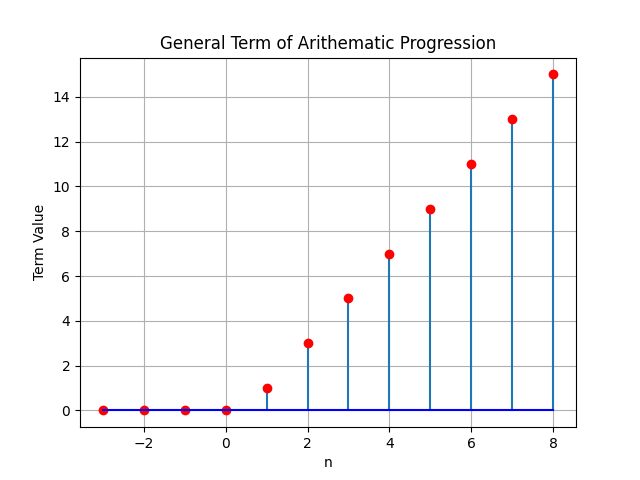
\includegraphics[width=1.0\linewidth]{Figure_2.png}
    \caption{Plot of general term of AP taken from Python}
    \label{fig:1}
\end{figure}
The Z-Transform Equation for x\brak{n} is 
\begin{align}
    X\brak{z}&=\sum_{n=-\infty}^{\infty}\brak{2n-1}z^{-n}u\brak{n} \\ \implies X\brak{z}&=\sum_{n=\infty}^{\infty}\brak{2n}z^{-n}u\brak{n} -\sum_{n=-\infty}^{n=\infty}z^{-n}u\brak{n}\\
   \implies X(z)&=2\sum_{n=0}^{\infty}\dfrac{n}{z^{n}}-U\brak{z}
\end{align}
\text{The first part of summation is}\\
\begin{align}
   \implies S_\infty&=\dfrac{z^2}{\brak{z-1}^{2}}
\end{align}
\text{The second part of summation is}\\
\begin{align}
   U\brak{z}=\dfrac{1}{1-z^{-1}}
\end{align}
The result is,
\begin{align}
    X\brak{z}&=2S_\infty-U\brak{z}\\
    X\brak{z}&=\dfrac{z^2}{\brak{z-1}^{2}}-\dfrac{1}{1-z^{-1}}\\
    X\brak{z}&=\dfrac{z^2+z}{\brak{z-1}^{2}}
\end{align}
(ROC) \(|z| > 1\).
\end{document}
